%
% Author: Daniel (dmilith) Dettlaff
%

\documentclass{beamer}
\usepackage{beamerthemeshadow}
\usepackage{graphicx}
\begin{document}
\title{Sofin + TheSS in action}
\author{Daniel (dmilith) Dettlaff}
\date{\today}

\frame{
  \titlepage
}

\frame{
  \frametitle{Table of contents}
  \tableofcontents
}

\section{Design solutions}
\subsection{Sofin with TheSS - In depth}
\frame{
  \frametitle{What is what}
    \begin{itemize}
    \item Sofin: The Software Installer
    \item TheSS: The Service Spawner
    \item /Software: root owned system wide utils and base system extension software.
    \item \textasciitilde/Apps: user owned software.
    \item \textasciitilde/SoftwareData: user software data.
    \end{itemize}
}

\frame{
  \frametitle{Terminology/ Glossary}
    \begin{itemize}
    \item Software definition: "def" file, with all info required to build software from scratch.
    \item Software bundle: software with all requirements - built from some definition and put inside /Software or \textasciitilde/Apps.
    \item Bundle exports: executables available for each software bundle.
    \item Binary build: prebuilt software available without need of compiling anything.
    \item Software igniter: "json" file, with info how to launch software with predefined settings.
    \end{itemize}
}


\frame{
  \frametitle{More details about roles}
    \begin{itemize}
    \item Sofin: apt-get - like command line util. `sofin install ruby' and you're done. If binary build is available, it will just download binary package and install it.
    \item TheSS: works as a user daemon, constantly watching pid files, and/ or service TCP port(s) for each software service. It's controled through \textasciitilde/SoftwareData/Softname/ igniter hooks (start, stop, restart, configure, ...) and indicators (starting, restarting, configuring, ...).
    \end{itemize}
}


\section{Examples}
\subsection{Switch between Ruby implementations}
\frame{
  \frametitle{Switch between Ruby implementations}

  \begin{block}{get latest Ruby bundle}
    sofin get ruby\\
    ruby -v\\
    ruby 2.0.0p195 (2013-05-14 revision 40734)\\
  \end{block}
  \begin{block}{get Ruby 1.8}
    sofin get ruby18\\
    ruby -v\\
    ruby 1.8.7 (2012-06-29 patchlevel 370)\\
  \end{block}
  \begin{block}{switch back to Ruby}
    sofin get ruby\\
    ruby -v\\
    ruby 2.0.0p195 (2013-05-14 revision 40734)\\
  \end{block}
}

\subsection{TheSS}
\frame{
  \frametitle{TheSS}

  \begin{figure}[ht!]
  \centering
  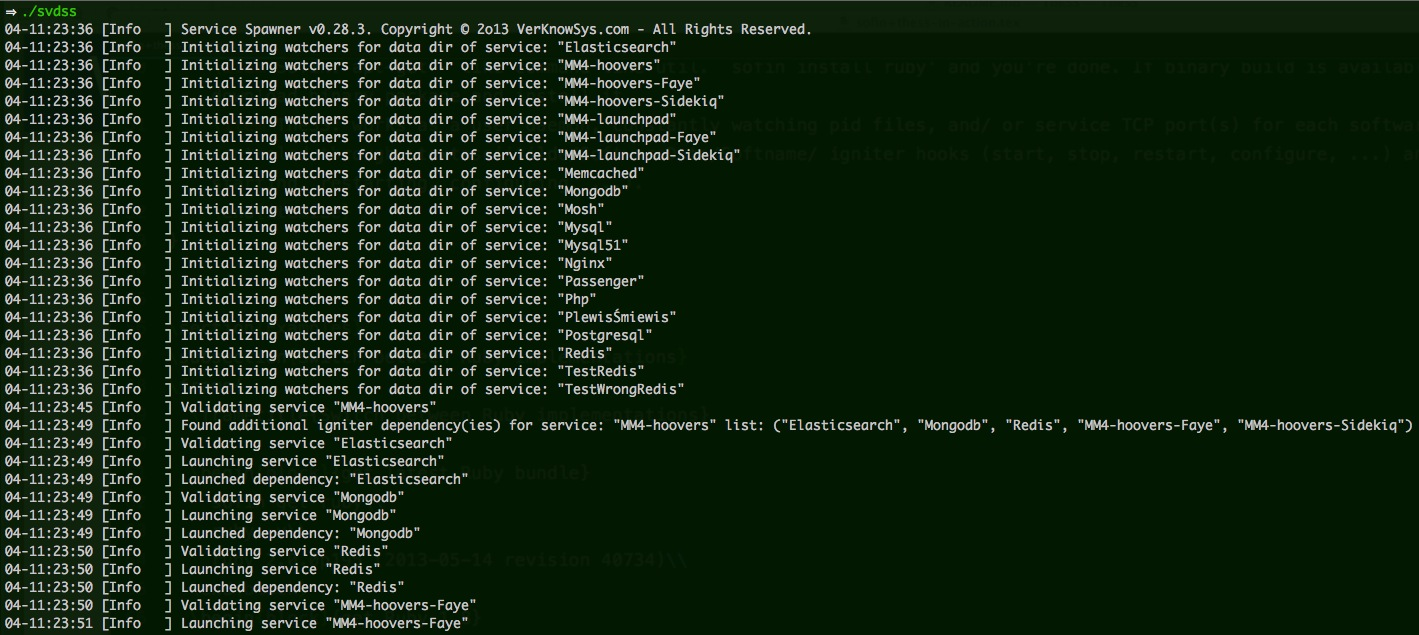
\includegraphics[width=115mm]{svdss.jpg}
  \caption{TheSS daemon in action}
  \label{overflow}
  \end{figure}
}

\subsection{TheSS UI panel}
\frame{
  \frametitle{TheSS UI panel}

  \begin{figure}[ht!]
  \centering
  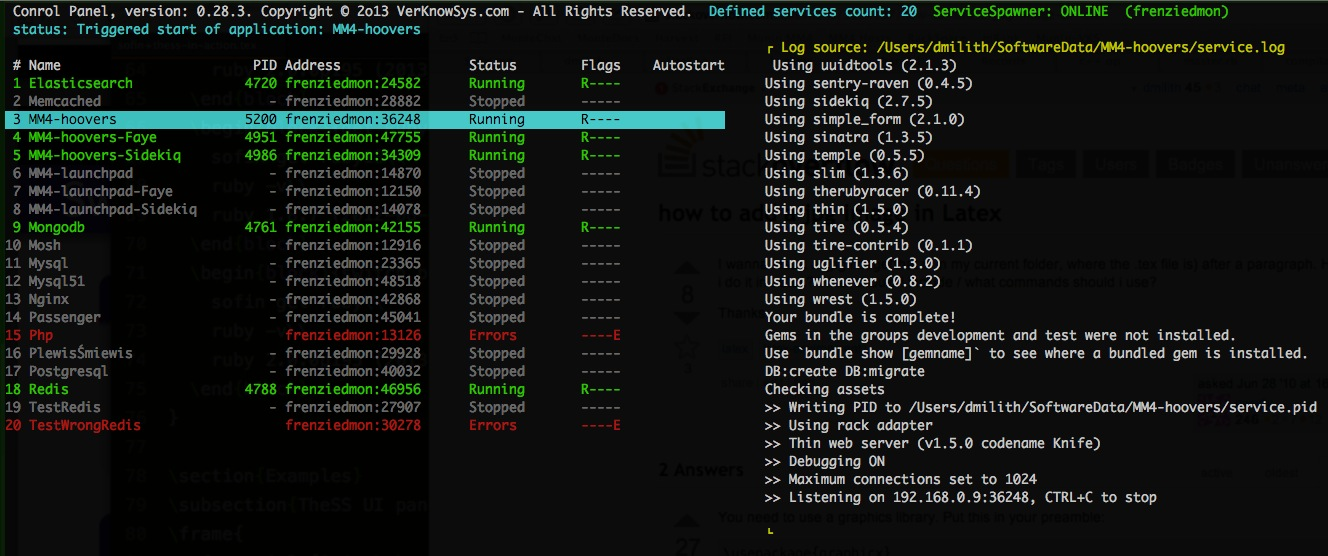
\includegraphics[width=115mm]{svdpanel.jpg}
  \caption{TheSS control panel UI in action}
  \label{overflow}
  \end{figure}
}

\section{Where and how?}
\subsection{Project pages}
\frame{
  \frametitle{Project pages}

  \begin{itemize}
    \item I'm \href{mailto:dmilith@verknowsys.com}{dmilith@verknowsys.com}, dmilith on Twitter
    \item https://github.com/VerKnowSys/sofin - Sofin
    \item https://github.com/VerKnowSys/TheSS - TheSS
  \end{itemize}

}

\end{document}

